% !TEX root = ../../../main.tex
% 来源：中学数学实验教材·第三册（高中数学）
% 章节：函数及其图象 / 一次函数（线性函数）
% 原始文件：4.tex，行 1227-1235
% 类型：tikz
% ---
    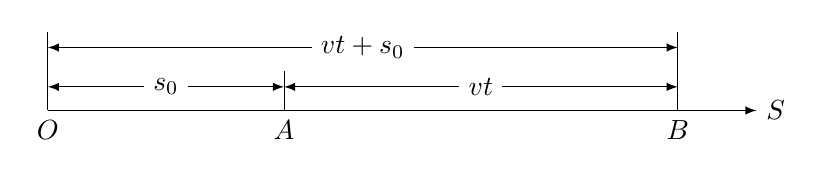
\begin{tikzpicture}[>=latex]
    \draw[->] (0,0)--(9,0)node[right]{$S$};
    \draw (0,0)node[below]{$O$}--(0,1);
    \draw (3,0)node[below]{$A$}--(3,.5);
    \draw (8,0)node[below]{$B$}--(8,1);
    \draw [<->] (0,.3)--node[fill=white]{$s_0$}(3,.3);
    \draw [<->] (8,.3)--node[fill=white]{$vt$}(3,.3);
    \draw [<->] (0,.8)--node[fill=white]{$vt+s_0$}(8,.8);
    \end{tikzpicture}
